\section{Crtanje proizvoljnih kontura}
\label{sec:Drawing}

Epiciklusi se mogu posmatrati kao krive definisane slede\'c{}im jedna\v{c}inama:
\begin{equation}
\begin{aligned} 
    x(t) & = \sum_i^N R_i\cos(\omega_i t + \phi_i)\\ 
    y(t) & = \sum_i^N R_i\sin(\omega_i t + \phi_i)\\ 
\end{aligned}
\label{eq:ep}
\end{equation}
gde $N$ predstavlja broj krugova u epiciklusu, $R_i$ predstavlja radijus kruga $i$, $\omega_i$ predstavlja ugaonu brzinu pridru\v{z}enu krugu $i$, a $\phi_i$ ozna\v{c}ava za koliki ugao je krug $i$ zarotiran u trenutku $t = 0$ (u daljem tekstu \emph{fazni pomeraj}).

Postavlja se pitanje: \emph{Kakve sve oblike, tj. orbite, mo\v{z}emo opisati epiciklusima}? Iz odeljka \ref{sec:Epicycles} znamo da se bilo kakva neprekidna linija mo\v{z}e opisati epiciklusom, pa \v{c}ak i prave linije ukoliko su krugovi istih dimenzija i rotiraju se u suprotnim smerovima tako da se $y$ komponente poni\v{s}tavaju (videti sliku \ref{img:line}). Jedini problem je zapravo odrediti vrednosti za $R$, $\omega$ i $\phi$ tako da prate proizvoljnu orbitu.

\begin{figure}
    \centering
    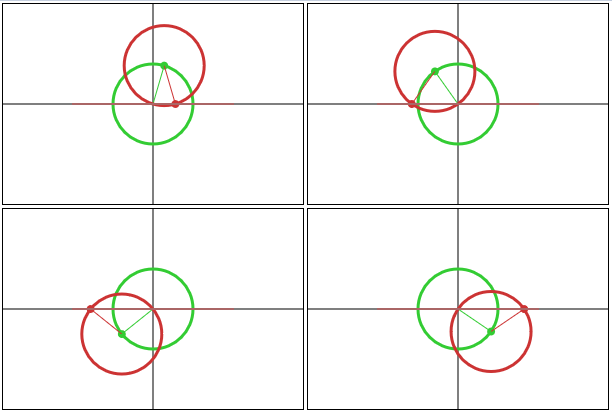
\includegraphics[scale=0.7]{images/line.PNG}
    \caption{Iscrtavanje prave linije zahteva samo dva kruga.}
    \label{img:line}
\end{figure}


\subsection{Ra\v{c}unanje epiciklusa za datu orbitu}

Najpre formalizujmo problem. Signal je dostupan u diskretnom obliku, kao skup ta\v{c}aka $(x_j,y_j)$. Zadatak je prona\'c{}i epicikluse tako da se date ta\v{c}ke najbolje spoje. Ta\v{c}nije, tra\v{z}imo $R_i$, $\omega_i$ i $\phi_i$ tako da $x(t)$ i $y(t)$ iz jednakosti \ref{eq:ep} \v{s}to bli\v{z}e odgovaraju signalu. $R_i$, $\omega_i$ i $\phi_i$ se onda mogu dobiti re\v{s}avanjem odgovaraju\'c{}eg sistema jedna\v{c}ina.

Prime\'c{}ujemo da u formalizaciji problema moramo \emph{pribli\v{z}iti} aproksimaciju signalu. To se mo\v{z}e formalizovati na razne na\v{c}ine, naj\v{c}e\v{s}\'c{}e pojmom \emph{srednjekvadratne gre\v{s}ke} \cite{NI}.

Ukoliko posmatramo ta\v{c}ke kao kompleksne brojeve, mogu\'c{}e je iskoristiti Ojlerovu formulu,
$$e^ix = \cos x + i\sin x,$$
i DFT proceduru opisanu u \ref{sec:Fourier} kako bismo kreirali algoritam koji je veoma jednostavan za ra\v{c}unar. Najpre formirajmo kompleksni broj koriste\'c{}i jedna\v{c}ine \ref{eq:ep}:
$$p_j = x_j + iy_j \\ x(t) + iy(t) = \sum_i^N R_i(\cos(\omega_i t + \phi_i) + i\sin(\omega_i t + \phi_i)).$$

Prime\'c{}ujemo da nismo ni\v{s}ta izgubili prelaskom na kompleksnu reprezentaciju, naime $x$ i $y$ su zapravo realni i imaginarni deo komplesnog re\v{s}enja. Sada, uz pomo\'c{} Ojlerove formule, shvatamo da tra\v{z}imo promenljive takve da izraz
$$\sum_j^N R_je^{i\omega_j t+ \phi_j}$$
\v{s}to bli\v{z}e odgovara kompleksnim brojevima $p_j$. \v{S}tavi\v{s}e, ukoliko dozvolimo da $X_j$ bude kompleksan broj, izraz postaje:
$$\sum_j^N X_je^{i\omega_j t}$$

Radi simplifikacije, umesto biranja $N$ ugaonih brzina $\omega$, postavi\'c{}emo fiksne brzine: $0, 1x, -1x, 2x, -2x, \dots , N/2x, -N/2x$. Sa ovom pretpostavkom, problem poprima finalni oblik:

\begin{prob}
    Prona\'c{}i kompleksne brojeve $X_j$ (krugove epiciklusa) minimizuju\'c{}i srednjekvadratnu gre\v{s}ku izmedju kompleksnih ta\v{c}aka $p_j$ i krive
    $$p(t) = \sum_{j=0}^N X_je^{\frac{2\pi i j}{N}t}.$$
\end{prob}

Problem opisan iznad skoro u potpunosti odgovara DFT formi. Stoga, dovoljno je iskoristiti DFT algoritam (videti \ref{sec:appendix:dft}), dobiti kompleksne brojeve $X_j$ i zatim izra\v{c}unati nepoznate parametre:
$$R_j = |X_j|,$$
$$\omega_j = \frac{2 \pi i j}{N},$$
$$\phi_j = \arctantwo(\Im{X_j}, \Re{X_j}).$$
